\documentclass[12pt]{article}
\usepackage{geometry}
\geometry{a4paper}
\usepackage[colorlinks, linkcolor=blue, citecolor=blue, urlcolor=blue]{hyperref}
\usepackage[automake]{glossaries-extra}
\usepackage{appendix}
\usepackage{graphicx} % Needed for including images
\usepackage{mdframed} % For creating framed boxes
\usepackage[backend=biber, style=ieee]{biblatex} % Adding biblatex with IEEE style
\usepackage{setspace} % 导入setspace包以控制行距
\usepackage{minted}
\usepackage{array}
\usepackage{glossaries}
\usepackage{multicol}
\addbibresource{Reference.bib} % Specify the bibliography file, here 'references.bib'


\makeglossaries % Initialize the glossary system

% Define some terms


\newabbreviation{davinci}{da Vinci Platform}{
    da Vinci Platform
}
\newabbreviation{tcn}{TCN}{
    Temporal Convolutional Network 
}
\newabbreviation{onnx}{ONNX}{
      Open Neural Network Exchange
}
\newabbreviation{gcn}{GCN}{
      Graph Convolutional Network
}
\newabbreviation{ros}{ROS}{
    Robot Operating System
}
\newabbreviation{ots}{OTS}{
      Optical Tracking System}
\newabbreviation{emts}{EMTS}{
      Electromagnetic Tracking System}      
\newabbreviation{rmis}{RMIS}{
      Robot-assisted minimally invasive surgery}
\newabbreviation{pnp}{PnP}{
      Perspective-n-Point}
\newabbreviation{6dof}{6DoF}{
      Six Degrees of Freedom}
\newabbreviation{p3p}{P3P}{
      Perspective-3-Point}
\newabbreviation{epnp}{EPnP}{
      Efficient Perspective-n-Point
}
\newabbreviation{sift}{SIFT}{Scale Invariant Feature Transform}
\newabbreviation{surf}{SURF}{Speeded Up Robust Feature}
\newabbreviation{icp}{ICP}{Iterative Nearest Point}
\newabbreviation{mis}{MIS}{Minimally invasive surgery}

% Define an acronym




\begin{document}

\begin{titlepage}
      \centering

      
\includegraphics[width=0.8\textwidth]{Imperial_College_London_new_logo.png} % Increased width
      \vspace*{1cm}

      \Large
      SURG70006 Group Project

      \large
      2024/10

      \vspace{0.5cm}
      \Huge
      \textbf{Project 19 \\ Surgical Robot Instrument Pose Estimation Inception Report}

      \vspace{1.3cm}


      % Framed box for student information
      \begin{mdframed}
            \normalsize % Smaller text size within the box
            \textbf{Group Number:} Group 8\\[20pt] % Name on the same line, add vertical space
            \textbf{Group Members:} Jie Li, Jinling Qiu, Leen AIShelh, Yanrui Liu, Yulin Huang\\[20pt] % ID on the same line, add vertical space
            \textbf{Supervisors:} Dr Stamatia Giannarou, Haozheng Xu % Supervisor on the same line
      \end{mdframed}

      \vspace{2cm} % Adjust space as necessary
      \Large
      \textbf{Department of}\\
      \vspace{0.1cm} % Adjust line spacing
      \textbf{Surgery and Cancer}

      \vspace{3.6cm} % Large space as required
      \Large
      Imperial College London\\
      


\end{titlepage}

\newpage
\tableofcontents

\newpage

% Introduction & Background
\section{Introduction}
\subsection{Minimally Invasive Surgery and Robotic Surgery}
\gls{mis} has expanded significantly in modern medicine, driven by advancements in robotics and technology. \gls{mis} involves a surgeon using elongated instruments and a surgical camera inserted through small incisions, resulting in reduced trauma to the patient compared to open surgery\cite{mcafee2010minimally}\cite{allan20183}. Research indicates that \gls{mis} often leads to better outcomes, such as shorter patient recovery times and increased surgical efficiency\cite{mcafee2010minimally}. However, \gls{mis} is also limited by factors such as reduced tactile feedback and depth perception, which can complicate the surgeon’s tool manipulation and contribute to increased cognitive workload, especially when the surgeon relies solely on visual feedback\cite{allan20183}\cite{allan2017visual}. Moreover, the training process for new surgeons is lengthy, as it takes considerable time for them to master the techniques\cite{allan20183}\cite{allan2017visual}\cite{hein2021towards}.

To address the limitations of open surgery and \gls{mis}, \gls{rmis}, such as the da Vinci system, was developed with enhanced dexterity, additional degree of freedom, clearer 3D vision and cancels out tremors\cite{plerhoples2012aching}\cite{allan2017visual}\cite{allan20183}. This technology enables surgeons to perform procedures with minimal trauma to critical structures and provides a clear view of various pathologies\cite{allan2017visual}.

During \gls{mis}, the surgeon might have limited view due to instrument obstruction, which can negatively impact the outcome especially with the surgeon depending entirely on visual feedback \cite{kassahun2016surgical}. When instruments block the camera's line of sight, it can result in unexpected and unintended damage to adjacent tissues, possibly harming vital anatomical structures such as vessels, nerves or ducts. Consequently, this may result in longer surgeries, increased morbidity and potential long-term complications\cite{allan2017visual} \cite{allan20183}. Although the latest da Vinci model has haptic feedback, allowing surgeons to have force-related input\cite{saracino2019haptic}, the clinical implications are not fully understood. With that in mind, pose estimation can allow the surgeon to have more precise and intended movement during the surgery, reducing the percentage of iatrogenic injuries\cite{allan2017visual}\cite{hein2021towards}. Furthermore, the surgeon may experience a high cognitive load, causing mental and physical fatigue due to constant adjustment of camera and instrument position to maintain a clear view of the anatomy\cite{allan20183}\cite{allan2017visual}\cite{shugaba2022should}. This can divert the surgeon's attention to tasks other than the surgery. Therefore, recent research in estimating instrument position is being conducted as it “can enable skill analysis, phase detection, motion estimation, tool–tissue interaction and pave the way towards image-guided interventions”\cite{hein2021towards}. Nowadays there are many external devices like depth camera, electromagnetic trackers etc. available for space estimation in surgical instruments but they are not practical in in-vivo surgeries because of space and hardware constraints\cite{enhancedmarker}.

\subsection{Problem Statement}
There are some vision-based methods that use external markers to track the instruments. However, these methods have major limitations: the markers must always be visible in the camera's field of view and are sensitive to background changes and occlusions\cite{10160287}. In this case, a vision-based markerless instrument tracking method that does not require any modifications to the hardware setup or external markers is necessary. 
\subsection{Engineering Background}
The da Vinci surgical robot operates with \gls{6dof}. These \gls{6dof} refer to the robot's ability to move and rotate in three-dimensional space, including three translational movements (up/down, left/right, forward/backward) and three rotational movements (pitch, yaw, and roll)\cite{app9030546}. This range of motion allows the da Vinci system to replicate the complex dexterity of a surgeon's hand for precise control over surgical instruments in confined spaces. The main aim of this project is to develop a deep learning based markerless \gls{6dof} surgical instrument pose estimation system. The system will be designed to provide highly accurate surgical instrument \gls{6dof} estimation without relying on external markers or complex hardware. \gls{6dof} surgical instrument pose estimation with and without occlusion shown in Figure 1\cite{surgripe2024}.

\begin{figure}[H]
            \centering
            \includegraphics[width=0.8\textwidth]{6Dof.png}
            \caption{\gls{6dof} surgical instrument pose estimation with (left) and without occlusion (right)\cite{surgripe2024}}
      \end{figure}



Pose estimation refers to finding the transformation (translation and rotation) that relates the object (or camera) coordinates in 3D space to its projection on a 2D image. The pose estimation of surgical tools has emerged as a critical job in \gls{rmis}. The majority of robots in \gls{rmis} are driven by cables, resulting in kinematic input that is not always precise, since the kinematic data describes the positions of the motor rather than the real position of the joints connected to the motor via a cable\cite{10160287}. 

\gls{ots} and \gls{emts} are well-established methods for tracking in medical applications. \gls{ots} offers high accuracy but requires a clear line-of-sight, making it prone to errors when obstructed. \gls{emts}, while effective without line-of-sight, suffers from interference caused by metal objects and electronic devices in the operating room, leading to reduced accuracy\cite{8822749}.

In \gls{rmis}, a marker-based method involves placing artificial markers on surgical instruments to aid vision-based instrument tracking\cite{villani2021development}. These markers can often be easily recognised in complex surgical environments. However, if the markers are damaged or obscured by blood coverage, this may result in detection failure\cite{ma2021comprehensive}. In addition, markers on the surface of surgical instruments must meet sterility requirement\cite{xu2023graph}. To address these issues, marker-less methods have been gradually proposed\cite{reilink20133d}. Marker-less methods do not rely on artificial markers in endoscopic procedures, but rather on natural features of the surgical instruments for gesture estimation. This method does not require additional marking process for the instruments and is able to adapt to various environmental changes with higher flexibility. However, the current marker-less method still faces some challenges, such as being susceptible to interference from lighting conditions, blood occlusion, and instrument reflections, and may not perform as consistently as the marker-based method in complex scenes\cite{hein2021towards}.


\section{Related Work}
\subsection{Traditional Non-learning Methods}
Traditional non-learning pose estimation methods are based on geometric modeling, algebraic techniques, and computer vision approaches\cite{fan2024reinforcement}. Non-learning methods differ from deep learning methods, which require a large amount of data as input. Typically, the core of traditional non-deep learning methods is featuring extraction, which is used to obtain a unique representation of an object by identifying edges, key points, or regional features\cite{fan2024reinforcement}. In the early days, the main methods for feature recognition include \gls{sift}\cite{lakshmi2017image}, which is a classical local feature descriptor that helps machines to identify and match feature points in different images, and to find key points in different scale-spaces. Another is the \gls{surf}\cite{wijesinghe2010speed}, which is an improved variant of \gls{sift} that improves the performance of feature extraction by optimising the process of feature detection and description.

After feature extraction is completed, the target model needs to be parameterised. The  \gls{pnp} problem, introduced by Fischler in the 1980s, is a commonly used algorithm for model parameterisation. It focuses on estimating a camera's position and orientation using 3D-to-2D point correspondences \cite{Lu_2018}. \gls{p3p} solves this with three such correspondences, providing up to four solutions. \gls{pnp} handles larger datasets by representing n 3D points as a weighted sum of four virtual control points, reducing computational complexity \cite{10.1007/s11263-008-0152-6}. Another method is the \gls{icp} algorithm\cite{bellekens2014survey}, which computes the pose relationship between two-point clouds by minimising the distance between corresponding points. Another method is the \gls{icp} algorithm\cite{bellekens2014survey}, which computes the pose relationship between two-point clouds by minimising the distance between corresponding points.
Non-learning methods have better interpretability and can achieve more accurate results while saving computational resources. However, such methods are less robust when dealing with complex scenes and lighting changes and have certain limitations\cite{bellekens2014survey}.


\subsection{Deep Learning Method}
In recent years, deep learning has been gradually applied to the field of surgical instrument pose estimation. Different from the traditional way that relies on geometric models and manual feature extraction, deep learning methods can infer the complex relationship between points and points from a large amount of data \cite{ bellekens2014survey}. According to the facts, deep learning methods are more capable of handling complex scenes with lighting changes\cite{fan2024reinforcement}. Through the concern classification of the model, it can be divided into holistic methods and intermediate representation method.

\subsubsection{Holistic Methods}
The holistic methods extract estimated surgical instrument poses by modelling global features of the entire scene\cite{fan2024reinforcement}. This approach does not rely on local detail features, but rather extracts pose information from global features making the holistic methods highly robust to complex scene variations. In 2015, Alex Kendall and his team proposed PoseNet, a deep learning method that directly regresses camera pose from monocular RGB images, enabling end-to-end position and orientation end-to-end estimation\cite{kendall2015posenet}. In 2020, Yannick Bukschat et al. proposed EfficientPose, an end-to-end 6D multi-target pose estimation method. The model is capable of simultaneously detecting the 2D bounding boxes of multiple targets in a monocular image and regressing their complete 6D poses in 3D space\cite{bukschat2020efficientpose}. In 2022, Bo Chen and colleagues developed the ROPE framework, which introduces a new occlusion enhancement technique and a multi-precision supervised mechanism, aiming to learn deep features that are robust to occluded environments, thus improving the accuracy of pose estimation in object-occluded scenes\cite{chen2022occlusion}.

The holistic methods are able to capture the overall features of an object directly from the whole image, with low dependence on feature points, without the need for precise positioning of feature points or additional feature extraction steps, which makes the model structure more concise\cite{chen2022occlusion}. However, the holistic methods are less accurate in dealing with local details, and when surgical instruments are occluded, it is difficult to recover the occluded instrument information from the overall features\cite{watson2014nature}.

\subsubsection{Intermediate Representations}
The intermediate representation method decomposes the complex pose estimation task into multiple more manageable subtasks by introducing a finer-grained intermediate description of the target. By extracting local features, the method effectively solves the problem that it is difficult to accurately estimate the pose of surgical instruments when they are occluded\cite{song2020hybridpose}.

In 2017, Yu Xiang and his team proposed PoseCNN for pose estimation in complex scenes. The method decomposes the pose estimation task into multiple components that deal with 3D translations and rotations of images separately. In addition, PoseCNN introduces a novel loss function that allows the network to better handle objects with symmetry\cite{xiang2017posecnn}.

Subsequently, in 2019, Sida Peng and his team proposed PVNet\cite{peng2019pvnet}. This approach uses a pixel-level voting network that significantly improves pose estimation accuracy in occluded and truncated scenes by predicting vectors from each pixel to a key point, combined with a RANSAC-based voting mechanism.

In 2020, Masakazu Yoshimura and his team developed a deep learning model based on an improved SSD-6D architecture\cite{yoshimura2020single}. The model utilises a manually generated dataset of single-frame endoscopic images combined with data enhancement techniques to effectively address occlusion and perspective distortion problems common in surgical environments.

In 2022, Mitchell Doughty and his team proposed HMD-EgoPose\cite{yoshimura2020single}. The method uses the EfficientDet-D0 network for multi-scale feature extraction and combines rotational, translational, and hand sub-networks to achieve 6-degree-of-freedom markerless pose estimation in monocular RGB images.

In 2024, Jihun Park and his team introduced a new occlusion-aware loss function based on the YOLOv8 model, which dramatically improved the accuracy of precise detection and pose estimation of key points of surgical instruments in complex occlusion environments\cite{park2024towards}. The research team trained the model on a real surgical dataset, which significantly improved its robustness in real surgical scenarios.

The intermediate representation method makes the task much less difficult by decomposing the complex pose estimation task into multiple, more manageable subtasks. At the same time, intermediate representation models local features so that the model can still maintain high stability in complex scenes. However, this method requires high accuracy in data labelling, and the accumulation of errors may affect the accuracy of the final results due to the inclusion of multiple intermediate steps\cite{xu2023graph}\cite{allan20183}.


\section{Goals and Objectives}
\subsection{Objectives of the Project}
This project aims to leverage state-of-the-art deep learning models for pose estimation to accurately determine the rotation and position of surgical instruments present in the surgical environment during \gls{rmis}. The detailed objectives of the project are as follows:

\begin{enumerate}

\item \textbf{Dataset Analysis}
\\The first objective is to analyze the datasets which include high-quality images captured by the da Vinci Si endoscopic stereo camera and accurate ground truth data obtained from the Hamlyn Centre.

\item \textbf{Model Conversion}
\\This project will convert the PyTorch model to an \gls{onnx} model to enable its deployment on ARM architectures, such as the NVIDIA Jetson AGX platform.



\item \textbf{Robust Pose Estimation}
\\This project also needs to devise novel approaches to ensure accurate and robust pose estimation in the presence of challenges such as partial tool visibility, occlusions, and other variations encountered during surgery. 

\item \textbf{Performance Evaluation}

Finally, the project will evaluate and validate the performance of the applied models under various degrees of occlusion, ensuring their reliability in practical surgical scenarios.

\end{enumerate}



\section{Proposed Methodology}
\subsection{Model for Pose Estimation}
The proposed methodology employs a two-stage approach consisting of a keypoint prediction module and a spatio-temporal keypoint refinement module\cite{xu2023graph}.

In the keypoint prediction module, real-time video serves as input, and a ResNet18 network, pre-trained on the ImageNet dataset, is used as the backbone to extract image features. A segmentation branch is then applied to distinguish surgical tools from the background. Once segmented, a vector pixel voting process utilizes a vector field to predict the keypoint locations of the surgical tool\cite{xu2023graph}.

Following keypoint prediction, graph information is constructed for the identified keypoints. Temporal information is first captured using a \gls{tcn}\cite{zeng2020srnet}, which models the relationships between consecutive frames. Then, a \gls{gcn}\cite{yan2018spatial} extracts spatial relationships among the keypoints, refining their positions based on the graph structure\cite{xu2023graph}. The final 2D keypoint outputs from the model are subsequently converted into 3D coordinates using the \gls{pnp} algorithm\cite{yun2017object}.


\subsection{Model Conversion}
In the process of deploying deep learning models on the NVIDIA Jetson AGX platform, PyTorch models first need to be converted to the \gls{onnx} format to ensure cross-platform compatibility. The \gls{onnx} format is a common intermediate representation that enables model migration and transforming between different frameworks and hardware, so that PyTorch models can be used directly in the embedded environment. \gls{onnx} models can be optimized on the NVIDIA Jetson AGX through TensorRT. TensorRT can improve the inference speed and computational efficiency, especially for embedded platforms. This optimization process includes multi-threading, pipelining, buffer assignment, and network duplication\cite{Jeong2022TensorRTBasedFA}\cite{karumbunathan2022nvidia}. In addition, the use of docker containers for model deployment is required, enabling easy transformation of the model training environment for deploying complex models\cite{10283807}.


\subsection{Model Integration with da Vinci}
This system incorporates two visual subsystems(shown in Figure 2)\cite{7989412}. The endomicroscope system generates a high-resolution, large-area 2D mosaic by integrating multiple microscopic images. The stereo laparoscope system captures 3D spatial information through stereoscopic imaging. These two visual systems enable high-resolution 3D imaging and precise pose estimation. Initially, the system feasibility is verified using a marker-based method for pose estimation, followed by the implementation of a marker-less approach to generate accurate 3D coordinates. Trajectory planning is performed by combining the 3D coordinate information with the stereoscopic data from the Stereo Laparoscope System, ultimately achieving visual control to adjust the probe’s pose dynamically. The dVRK-ROS bridge establishes a connection between the dVRK system and the ROS (Robot Operating System). The CISST/SAW controller then operates the dVRK controller, enabling continuous control of the da Vinci robot.

\begin{figure}[H]
            \centering
            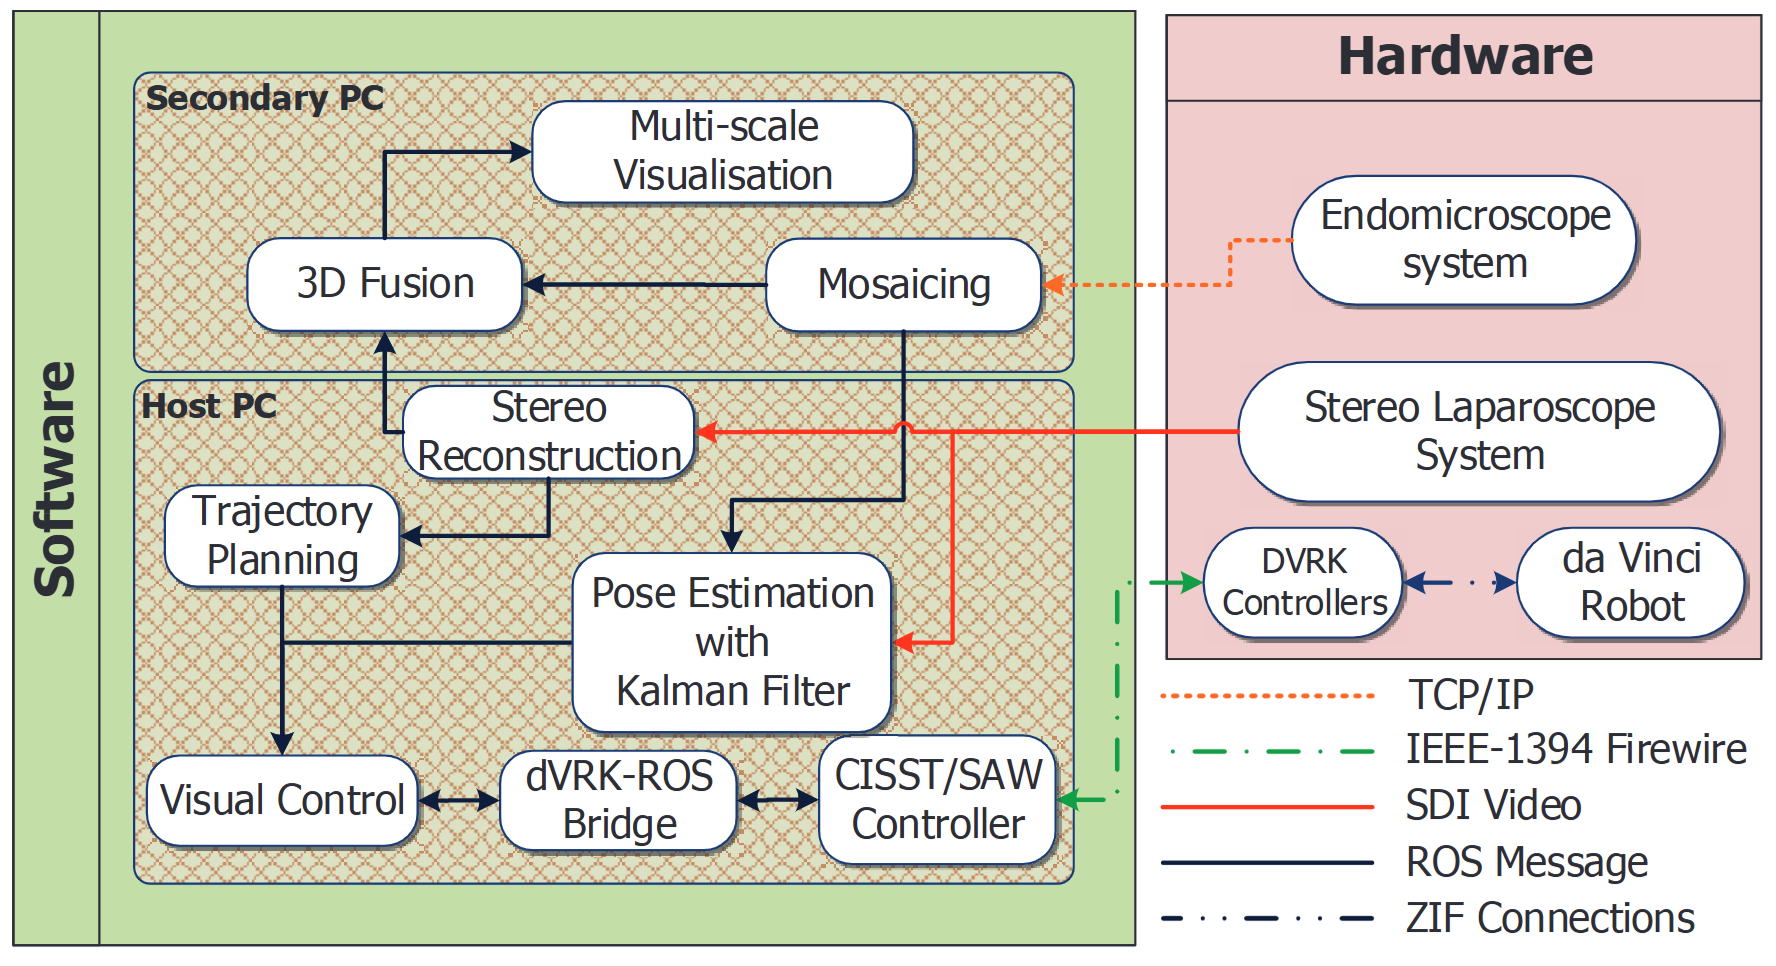
\includegraphics[width=0.7\textwidth]{model integration.png}
            \caption{An overview of the proposed system framework for autonomous endomicroscopic scanning and 3D mosaicing\cite{7989412}}
      \end{figure}



\subsection{Hardware and Software Requirements}
\textbf{NVIDIA Jetson AGX Platform Development}: This project will use NVDIA AGX Platform to deploy the deep learning models.\\
\textbf{Languages}: Python, C, C++ \\
\textbf{Tool Packages}: PyTorch, OpenCV \\
\textbf{ROS (Robot Operating System)}: A flexible framework for developing and running robot software across multiple systems. \\
\textbf{Docker}: A platform for deploying and managing applications in lightweight containers using OS-level virtualization.


\section{Project Timeline}
\begin{figure}[H]
            \centering
            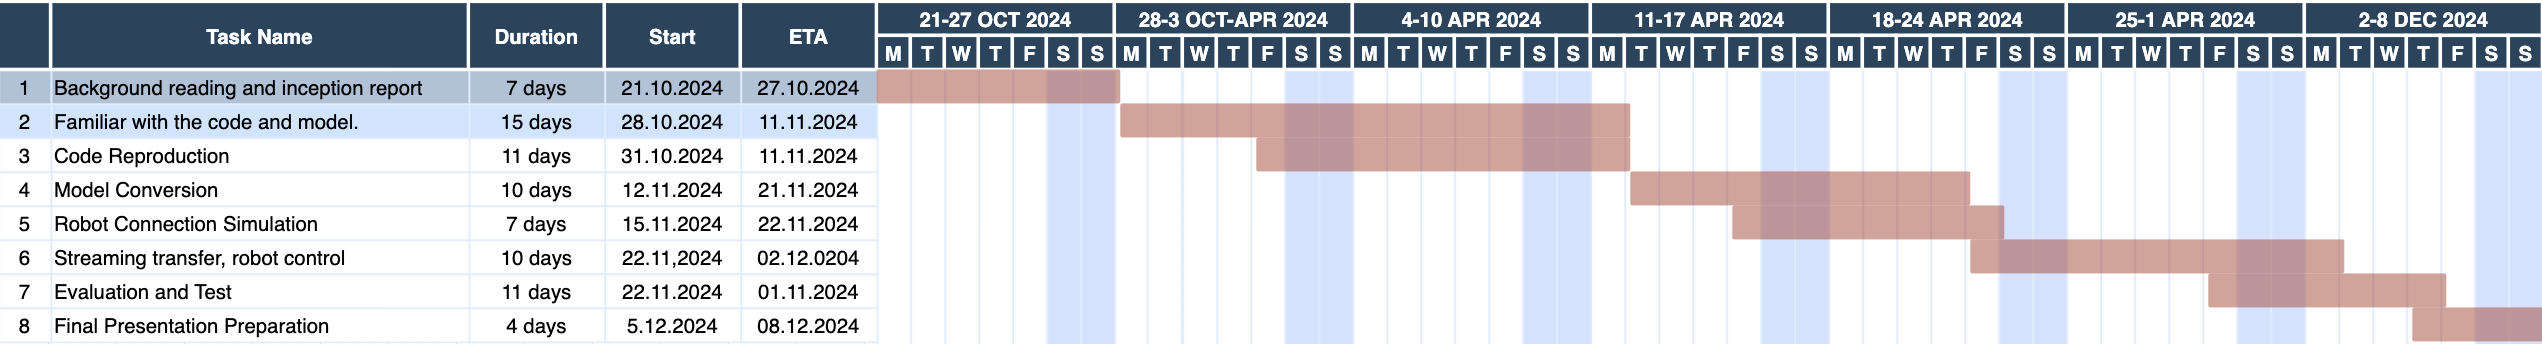
\includegraphics[width=\textwidth]{timeline.png}
            \caption{Gantt Chart}
      \end{figure}
      
\section{Risk Assessment}
\begin{table}[H]
      \centering
      \renewcommand{\arraystretch}{1.5} 
      \resizebox{\textwidth}{!}{
      \begin{tabular}{| >{\centering\arraybackslash}m{4cm} | >{\centering\arraybackslash}m{5cm} | >{\centering\arraybackslash}m{2.5cm} | >{\centering\arraybackslash}m{2.5cm} |}
      \hline
      \normalsize\textbf{Risk} & \normalsize\textbf{Mitigation Strategy} & \normalsize\textbf{Likelihood} & \normalsize\textbf{Impact} \\ 
      \hline
      \normalsize Pose estimation unstable in complex scenes (e.g., occlusion, dynamic background) & \normalsize Optimizing the dataset with more occlusion scene data & \normalsize High & \normalsize Very High \\ 
      \hline
      \normalsize Low frame rates & \normalsize Optimizing model efficiency and investing in high-quality hardware & \normalsize High & \normalsize Medium \\ 
      \hline
      \normalsize Model computation time is too long for real-time simulation & \normalsize Optimizing model efficiency and using hardware acceleration & \normalsize High & \normalsize Medium \\ 
      \hline
      \normalsize Reliance on specific deep learning frameworks, leading to migration difficulties & \normalsize Reducing binding to specific frameworks & \normalsize Medium & \normalsize High \\ 
      \hline
      \normalsize Data damage or lost & \normalsize Using GitHub or external storage devices to make backup & \normalsize Medium & \normalsize Very High \\ 
      \hline
      \normalsize Data privacy & \normalsize Implementing robust data encryption and complying with data protection laws such as GDPR & \normalsize Medium & \normalsize Very High \\ 
      \hline
      \normalsize Ethical and regulatory & \normalsize Consulting with regulatory experts and following related regulations & \normalsize Very Low & \normalsize High \\ 
      \hline
      \normalsize Timeline delay & \normalsize Making a detailed timeline and a thorough monitoring plan & \normalsize High & \normalsize High \\ 
      \hline
      \end{tabular}
      }
      \caption{Risk Assessment Table}
\end{table}


\section{Project Management}
\subsection{Progress Monitoring}
For the code part, we use GitHub for monitoring and progress management. We use GitHub's version control to branch the code (each team member manages a branch independently) to ensure smooth team collaboration. We also manually record project logs(such as meeting minutes and group activities) and combine them with timelines to ensure the project runs smoothly.
\subsection{Rules of Group Members}
\begin{table}[H]
      \centering
      \renewcommand{\arraystretch}{1.2} % 减少行距
      \resizebox{\textwidth}{!}{
      \begin{tabular}{| >{\centering\arraybackslash}m{4cm} | >{\arraybackslash}m{10cm} |}
      \hline
      \normalsize\textbf{Names} & \normalsize\textbf{Roles} \\ 
      \hline
      \normalsize Jinling Qiu (Leader) and Jie Li  & \normalsize Run samples on ROS and DVRK; Test arm movement with a given trajectory; Use marker-based pose to guide the instrument arm; Use the poses transferred from image processing group to guide the instrument arm, and Presentation Preparation \\ 
      \hline
      \normalsize Yanrui Liu, Yulin Huang and Leen AlShelh  & \normalsize Connect Real-time video stream from da Vinci endoscope to AGX; Deploy deep learning model on AGX (in pytorch or ONNX); Create pipelne for Real-time inference; use TCP-IP to send visual feedback to robotic control group, and Presentation Preparation \\ 
      \hline    
      \end{tabular}
      }
      \caption{Roles of Team Members}
\end{table}





% References (The bibliography will be printed here)
\renewcommand*{\bibfont}{\footnotesize} % 可以替换为 \footnotesize 或更小
\printbibliography

\renewcommand{\glossarypreamble}{\footnotesize \begin{multicols}{2}}
\renewcommand{\glossarypostamble}{\end{multicols}}

\printglossaries
\label{sec:glossary}

\end{document}
